\documentclass[class=jreport, crop=false, preview=false, dvipdfmx, a4paper, 14Q, fleqn]{standalone}
\usepackage{../../preamble/preamble_TeXManual}
\begin{document}

\chapter{ファイルの分割と統合}
\label{ch:file-management}

文書の量が多くなると,
どこに何が書いてあるのかわかりづらくなり,
1つの{\TeX}ファイルで管理することが難しくなります。
そこで,1つの文書を小分けにして別々で管理し,
また別のファイルで統合する,
という方法を紹介しておこうと思います。



\section{ディレクトリとパス}
\label{sec:path-and-directory}
ファイルを分け,統合するにあたって,
ディレクトリとパスというものを知っておく必要があります。
以下の小節でそれぞれ説明します。
知っている人は読み飛ばしてもらって構いません。


\subsection{ディレクトリ}
ディレクトリとは,色々なファイルを入れてあるフォルダのことです。
ファイルを人だと考えれば,
ディレクトリは家のようなものです。
ディレクトリは入れ子(多層構造)にすることができます。
例えば,日本というディレクトリに東京都というディレクトリがあり,
その中に23区のディレクトリがあり,
その中に本郷三丁目というファイルがある,
といった感じです。
このように,層の下に入っていく(狭い範囲になっていく)ことを「下に行く」,
逆に広い範囲を含む方へ行くことを「上に行く」ということにします。


\subsection{パス}
パスとは,そのファイルがコンピューターのどこにあるか,
という住所のようなものです。
パス(住所)を指定することで,
目的のファイル(人)を探し出して使うことができるようになります。

パスには「絶対パス」と「相対パス」の2種類があります。
絶対パスは,一番大元のディレクトリからスタートして指定するものです。
住所に例えれば,\\
\hspace{5zw} 宇宙 $\rightarrow$ 地球 $\rightarrow$ ユーラシア大陸 $\rightarrow$ 
アジア $\rightarrow$ 日本$\rightarrow$ 関東 $\rightarrow$ 東京 $\rightarrow$ 文京区 \\
のような感じです。
例えば,僕のPC上でこの \TeX マニュアルは,\\
\hspace{5zw} \verb|C:/Users/User/Document/TeX/TeXManual| \\
というところにあります。
この「Users」が,僕のPCの大元の
ディレクトリとなっています。

相対パスは,今いるところからの相対位置で指定するものです。
住所に例えれば,東京都から東京都に手紙を出すときに,
「東京都」の部分を省略して区名から書けばOK,
のような感じです。
相対パスを指定するとき,
同じディレクトリにあるファイルを指定するときはただそのファイル名を書けばよく, 
今いる(使っているファイルのある)ディレクトリより下のディレクトリのファイルを指定するときは,
「ディレクトリ名/ファイル名」とし,
今いるディレクトリより上のファイルを指定するときは「../ファイル名」とします。
上や下に行った数だけ「/」が書かれることになります

ここで,windowsではパスの区切りが円マーク(¥)や
バックスラッシュ(\verb|\|)となっていますが,
{\TeX}でのパスの区切りは全てスラッシュ(/)ですので,
注意してください。



\section{\TeX 標準のコマンド}
{\TeX}には,\verb|\input{.texファイル}|と\verb|\include{.texファイル}|
という2つのコマンドが用意されています。
この2つはともに,元の.texファイルのそのコマンドを,
指定された.texファイルの内容で置き換える,
というものとなっています。
違いとしては,\verb|\include|は改ページあり,
\verb|\input|は改ページ無し,となっています。
ちなみに,ファイル名の.texは省略できます。



\section{具体例}
色々解説してきましたが,
実際どのようにするのか見ないと
かなりわかりづらいと思うので
具体例を示します。

前書き,目次,第1~3章から構成された1つの文書を
異なるファイルに分割し,
統合することを考えます。
まずはフォルダを1つ作って,
前書き(maegaki.tex),
第1~3章(chapter1~3.tex)と,
文書に関連するファイルを全てその中に入れます
(ここではフォルダ名をexampleとします)。
図があるときはまとめてfguresフォルダにでも入れておきましょう。
また,プリアンブル(\verb|\documentclass|と\verb|\begin{document}|の間)も
分けて別の.texファイルに書きます(preamble.texとします)。
最後に統合用の.texファイル(main.tex)も同じ所に置いて準備完了です。
いま,exampleフォルダの中身は以下のようになっています。

\begin{figure}[H]
\begin{center}
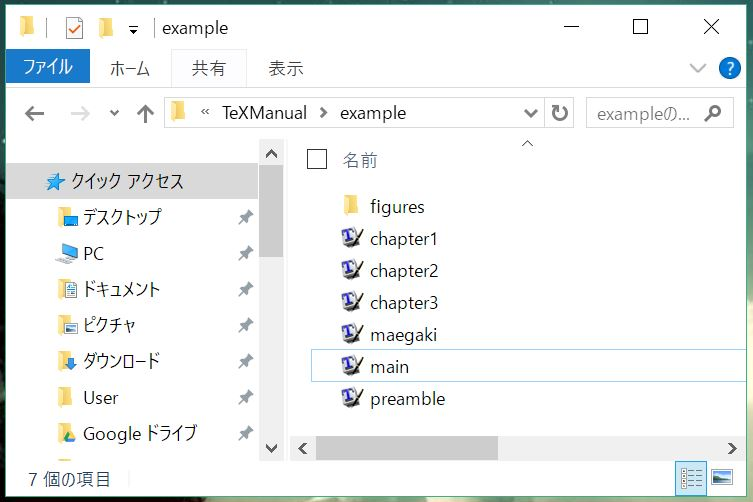
\includegraphics[width=10cm]{figures_for_file_management/directory_example1.jpg}
\end{center}
\label{fig:directory_example1}
\end{figure}

さて,次はmain.texの中身を見てみましょう。
\verb|\tableofcontents|は目次を出力するコマンドであることに注意してください。

\begin{ITeX}
\documentclass[dvipdfmx, a4paper]{jsarticle}
\usepackage{import}
\begin{document}
\tableofcontents
\include{maegaki}
\include{chapter1}
\include{chapter2}
\include{chapter3}
\end{document}
\end{ITeX}

mainでは分割したファイルを\verb|\include|を使って統合しています
(\verb|\include|は改ページを伴うので,
改ページしたくないときは\verb|\input|を使ってください)。
これでmainを実行すれば,
これらを全部一緒の.texファイルに書いたときと同じ出力が得られます。

なお,前節で説明した通り,\verb|\include|や\verb|\input|は
読み込んだ.texファイルをそこに書き写すだけなので,
読み込むファイル(preamble,maegaki,chapter1~3)には
\verb|\documentclass|~\verb|\begin{document}|,\verb|\end{document}|
は書かないでください。

この文書を書いている途中は,chapter3が用意されていなかったりすると思います。
また逆に,chapter2を書いているときは,
目次やchapter1は不要になるかもしれません。
そのときは,\verb|\include|コマンドの前に{\%}をつけてコメントアウトしてください。



\section{importパッケージの利用}
上では.texファイルを全て同じフォルダに入れていますが,
図が多かったりするときは章ごとにフォルダを作り,
その中に図のフォルダを作ることもあるかもしれません。
そのとき,フォルダの中身は例えば以下のようになるでしょう。

\begin{figure}[H]
\begin{center}
\begin{subfigure}{0.45\columnwidth}
	\begin{center}
	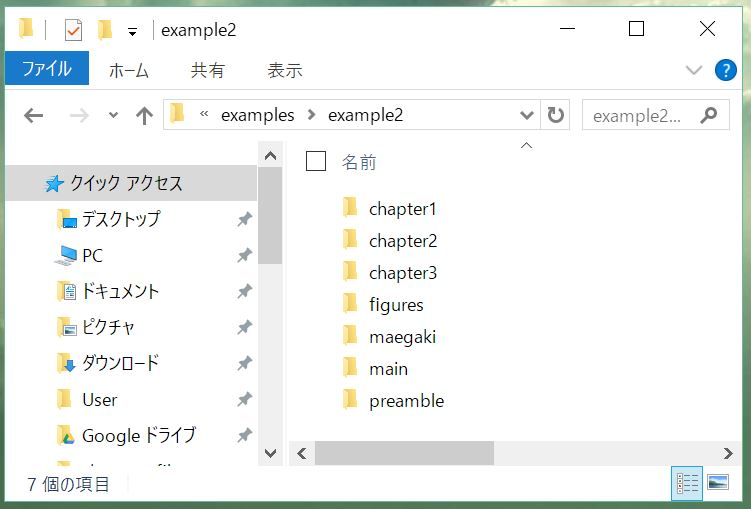
\includegraphics[width=\columnwidth]{figures_for_file_management/directory_example2.jpg}
	\end{center}
	\label{fig:directory_example2}
\end{subfigure}
\begin{subfigure}{0.45\columnwidth}
	\begin{center}
	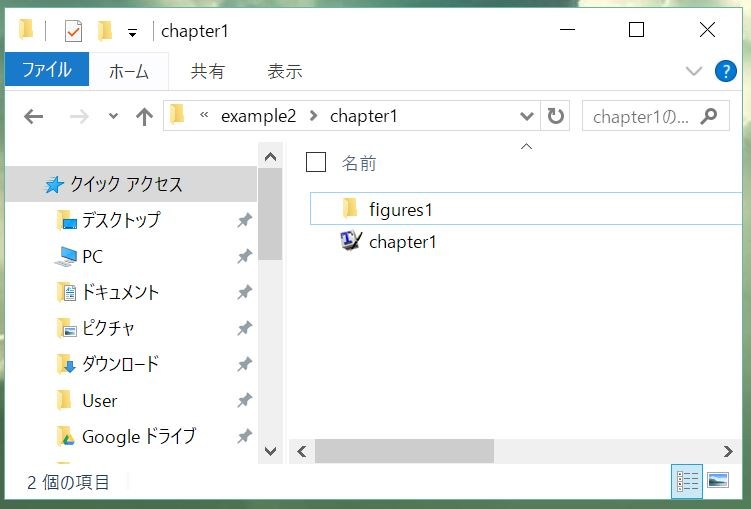
\includegraphics[width=\columnwidth]{figures_for_file_management/directory_example3.jpg}
	\end{center}
	\label{fig:directory_example3}
\end{subfigure}
\end{center}
\end{figure}

このとき,例えばchapter1をmainで\verb|\include|するには,
chapter1.texのパスを指定しなければなりません。
このパスは絶対パスでも相対パスでもいいですが,
mainからの相対パスで指定する方がよいと思います。
これは,絶対パスで指定すると,
後々mainのフォルダごと移動するときに全てのパスの指定を
書き直さなければならなくなるからです。
よって,main.texでは,
\begin{ITeX}
\include{../chapter1/chapter1.tex}
\end{ITeX}
のようにして読み込む形になります
(「../」は1つ上のディレクトリに移動することを表します)。

しかし,もしchapter1.texの中で\verb|\includegraphics|を使って
図を読み込んでいるなど,
他のファイルを読み込んでいる場合,
それがそのままmain.texに書き込まれる形になるので,
chapter1.texで書いた\verb|\includegraphics|の相対パスがずれてしまい,
結果図のファイルが見つからずエラーしてしまいます。

このとき,\verb|\include|でchapter1を読み込んでいる場合,
よくわからないエラーが出ます(多分解決不可です)。

もし\verb|\input|で読み込んでいる場合,
「!LaTeXerror file not found」的なエラーが出ます。
こちらは一応解決可能で,
chapter1.tex内で他のファイルを読み込んでいるところ
(\verb|\include|,\verb|\input|,\verb|\includegraphics|を使っているところ)
のパスの指定をmain.texからの相対パスに変更すれば解決できます。
しかしこの方法ではわかりづらい上,
mainを移動したりファイル名を変更したりしたときに
色々なところのパスをいじらなけばならず非効率的です。

よって,{\TeX}標準のコマンドだけでは,
フォルダ分けをしてファイルを管理する,
つまり\verb|\input|等の入れ子を扱うのが
非常に面倒です。

そこで,importという便利なパッケージを使います。
まずは\verb|\usepackage{import}|とプリアンブルに書きます。
このimportでは,
\begin{ITeX}
\import{絶対パス}{ファイル名.tex}
\subimport{相対パス}{ファイル名.tex}
\end{ITeX}
という2つのコマンドが定義されています。
この2つのコマンドでchapter1.texを読み込むと,
chapter1.tex内での\verb|\input|等は,
chapter1.texから見たパスとして扱われます。
したがって,mainから見た相対パスを考えてパスを書く,
といった面倒なことはなくなります。

また,これらのコマンドにはそれぞれ,
\verb|\inputfrom|,\verb|\subinputfrom|
という別名が用意されています。
なお,\verb|\import| と \verb|\subimport|
の2つを同じファイル内で使うとエラーするので気を付けてください。

このimportパッケージを使えば,
main.texの中身は以下のようになります。

\begin{ITeX}
\documentclass[dvipdfmx, a4paper]{jsarticle}
\usepackage{import}
\begin{document}
\tableofcontents
\subimport{../maegaki/}{maegaki}
\subimport{../chapter1/}{chapter1}
\subimport{../chapter2/}{chapter2}
\subimport{../chapter3/}{chapter3}
\end{document}
\end{ITeX}

これで,例えばchapter1.tex内で
\begin{ITeX}
\includegraphics{figures/fig1.pdf}
\end{ITeX}
のように,そこからの相対パスで図を読み込んでも
ちゃんとファイルを見つけてくれます。

このimportパッケージはファイルの分割時には非常に便利なので,
長い文書を書くときは是非使ってみて下さい。



\section{分割したファイルを実行する}
ここまでで,ファイルを分割してそれをまとめることはできるようになりました。
ただ,これだけだとちょっと不便です。
例えば,ファイルの一部を書き換え,
それを出力して修正するというとき,
その実行はmain.texを用いて行わなければなりません。
このとき,他のファイルごと実行すると実行時間がかなりかかりますが,
他のファイルを読み込んでいる\verb|\input|などをコメントアウトするのも面倒です。
そこで,分割したファイルを実行するやり方を紹介しようと思います。


\subsection{docmuteパッケージ}
docmuteパッケージを用いれば,
\verb|\input|と\verb|\include|されるファイルの
\verb|\begin{document}|と\verb|\end{document}|の外を無視し,
その中身だけを読み込むことができます。
まずはプリアンブル(preamble.tex)に
\begin{ITeX}
\usepackage{docmute}
\end{ITeX}
と書いてください。
ただ,このdocmuteパッケージはインストールされていない可能性もあります。
その場合は,第\ref{ch:packages}章\ref{sec:install-packages}節を見て
自分でインストールしてもよいですが,
後のstandaloneパッケージがほぼdocmuteの上位互換となっているので,
そちらを使ってもよいと思います。

使い方を説明します。
main.texの中身が以下のようになっているとします。

\begin{ITeX*}[title = main.tex]
\documentclass[dvipdfmx, a4paper]{jsarticle}
\usepackage{import}
\begin{document}
\include{../chapter1/chapter1}
\include{../chapter2/chapter2}
\include{../chapter3/chapter3}
\end{document}
\end{ITeX*}

また,chapter1.texの中身が以下のようになっているとします。

\begin{ITeX*}[title = chapter1.tex]
\documentclass[dvipdfmx, a4paper]{jsarticle}
\usepackage{import}
\begin{document}
\chapter{はじめに}
はじめに~~~~~。

\end{document}
\end{ITeX*}

まずはchapter1.texのみを実行し,内容を確認します。
内容がOKになったら,
main.texを実行します。
そうすると,\verb|\begin{document}|と\verb|\end{document}|の間だけがmainで読み込まれるので,
ファイルの統合もうまくいきます。

ここで注意ですが,プリアンブル部分は無視されるので,
main.texとchapter1.texのプリアンブルが異なっていると
それぞれの実行結果が変わる可能性があります。
できるだけ同じプリアンブルを使うようにしてください。
また,\verb|\include|と\verb|\input|は使えますが,
\verb|\import|や\verb|\subimport|は使えないので注意してください。



\subsection{subfilesパッケージ}
subfilesパッケージを使えば,
chapter1.tex等において親のmain.texのプリアンブルを引き継いで使うことができます。
まずはプリアンブル(preamble.tex)に
\begin{ITeX}
\usepackage{subfiles}
\end{ITeX}
と書いてください。

使い方ですが,chapter1.tex等のドキュメントクラスにsubfilesを指定し,
オプションでmain.texのパスを指定してください。
また,読み込みは\verb|\subfile|コマンドで行ってください。
具体的には,以下のようにするということです。

\begin{ITeX*}[title = main.tex]
\documentclass[dvipdfmx, a4paper]{jsarticle}
\usepackage{import}
\begin{document}
\include{../chapter1/chapter1}
\include{../chapter2/chapter2}
\include{../chapter3/chapter3}
\end{document}
\end{ITeX*}

\begin{ITeX*}[title = chapter1.tex]
\documentclass[../main/main.tex]{subfiles}
\begin{document}
\chapter{はじめに}
はじめに~~~~~。

\end{document}
\end{ITeX*}

こうすることによって,子のchapter1.texでmain.texのプリアンブルを読み込んで使うことができます。
プリアンブルを共有できるので,
いちいち子のファイルでプリアンブルを書いたり読み込んだりする必要がなくて便利です。

ただ,\verb|\import|や\verb|\subimport|に対応するコマンドは用意されていませんので注意してください
(僕が試したときは,chapter1.tex等で\verb|\input|を使うとテキストのみ読み込まれ,
tcolorboxやtikzが表示されないという形になりました)。

なお,この小節は
「\href{http://qiita.com/sankichi92/items/1e113fcf6cc045eb64f7}{分割したLaTeXファイルをsubfilesを使ってコンパイルする}」
を参考にしました。



\subsection{standaloneパッケージ}
standaloneパッケージを使えば,
子のプリアンブルを親に共有することができます。
まずは,subpreamblesオプションを追加して,
\begin{ITeX}
\usepackage[subpreambles=true]{standalone}
\end{ITeX}
としてください。

使い方ですが,main.texでの読み込みは\verb|\input|や\verb|\subimport|で行えます。
main.texの中身は上と同じとしますので,省略します。
子のファイルについてですが,
これは以下のようにします。

\begin{ITeX*}[title = chapter1.tex]
\documentclass[class=jsarticle, crop=false, preview=false, dvipdfmx, a4paper]{standalone}
\usepackage{import}
\newcommand{\kodomo}{子供}
\begin{document}
\chapter{はじめに}
はじめに~~~~~。
\kodomo

\end{document}
\end{ITeX*}

ドキュメントクラスにはstandaloneを指定し,
オプションでclass=jsarticle等とします。
jsarticle等につけるオプション(dcipdfmxやa4paper等)も普通につけることができます。
crop=flaseやpreview=falseですが,
僕はよくわからないまま使っているので是非自分で調べてみて下さい。

上の例では,chapter1.texのプリアンブルで\verb|\kodomo|というコマンドを定義し,
文章中でこれを使っています。
docmuteやsubfileではこれはmain.texには読み込まれないので,
main.texを実行するとエラーしてしまいます。
しかし,standaloneを使えば,子のプリアンブルが親にも共有されるので,
main.texを実行してもエラーしません。
他の子のファイルと共有しないようなプリアンブルは,
共有のプリアンブルでなく子のそれに書いてもよいでしょう。

standaloneパッケージでは,
\verb|\input|や\verb|\include|に加え\verb|\import|や\verb|\subimport|も使えるので,
これらを使いたい人はstandaloneパッケージを使ってみて下さい。

ここで注意ですが,子のプリアンブルが親のプリアンブルに共有されるので,
preamble.texの相対パスがmain.texからとchapter1.texからで異なる場合はエラーします。
絶対パスで指定してもいいですが,特に子のプリアンブルを親に共有しなくてもいい場合は,
\verb|\usepackage{standalone}|のように,
subpreamblesオプションを外してください。

このstandaloneパッケージは元々tikzという描画パッケージを読み込むときに便利なものです。
僕はその用途で使っているわけではないのであまりそちらには詳しくありません。
そちらの用途で使うとき用のオプションやコマンドが用意されているので,
是非自分で調べてみて下さい。

この小節は,
「\href{https://ja.sharelatex.com/learn/Multi-file_LaTeX_projects}{Multi-file LaTeX projects}」
を参考にしました。\\


上の全てのパッケージを通して,
子のchapter1.tex等で使った他ファイルへの参照となる\verb|\ref|は
「??」等となりうまく表示されません。
mainにおいてはちゃんと表示されるので
基本的にはそこまで気にしなくて大丈夫だと思いますが,
子のPDFをそのまま使う可能性がある場合は注意してください。


\end{document}